\section{Problema 2}
\indent Observación: Tuvimos problemas para implementar la lectura, resolución y escritura de un archivo, por lo que no presentamos la implementación de dicha funcionalidad en nuestro archivo $Tests2.java$.


\subsection{Resolución}

\subsubsection{Explicación del problema}
\indent El objetivo de este ejercicio es, dada un red de amistades y 2
investigadores, determinar cuántas veces el entusiasmo que se genera en uno de
ellos se verá fraccionado hasta, finalmente, generar un cierto entusiasmo en el
otro. \\
\indent Esto sucederá sólo en aquellos casos en los cuales estos investigadores
tengan amigos en común. En caso de existir varias redes de amistades
(entendiéndose por red de amistad a una conexión de amistades entre ambos
investigadores, sin que haya investigadores repetidos), se debe estudiar el caso
de la más corta, ya que esta red será la que generará el entusiasmo en el
investigador antes que cualquier otra y con la mayor proporción. \\
\indent Si no existiesen amigos en común entre ellos, es decir, si no existe una
red de amistad entre ambos, entonces el entusiasmo generado en uno nunca llegará
al otro, es decir la fracción de entusiasmo que le generará al investigador
destinatario será cero o, como se ha establecido, se indicará con $0$ la
cantidad de veces que éste se verá fraccionado.

\subsubsection{Primeros intentos de solución}
\indent En una primera aproximación al problema, pensamos en aplicar el
concepto de matrices de incidencia,
teniendo como índices a los investigadores por un lado y a las amistades por el
otro.\\
\indent Este clase de solución nos parecía productiva ya que al utilizar una
matriz, tanto para rellenarla en su totalidad como para recorrerla, los
algoritmos tienen una complejidad lineal O($m*n$), con $m$= cantidad de
amistades y $n$=cantidad de investigadores, quedando en evidencia que dicha
implementación cumplía la cota de complejidad pedida. \\
\indent Esta solución fue descartada una vez ya empezada su implementación.
Luego de buscar alguna estructura adecuada para representar a la matriz,
decidimos utilizar un diccionario de clave investigador y significado Lista de
amigos.\\
\indent El problema surgió a la hora de pensar un algoritmo para recorrer las
amistades con algún criterio y que no repita ninguna amistad. Luego de
contemplar varias opciones para tratar de solucionar este problema, nos dimos
cuenta de que estaba mal pensado el problema, ya que la matriz carecía de toda la
información relevante necesaria para realizar el algoritmo del recorrido de la
misma. Incluso sabiendo qué amistad se había recorrido, era difícil establecer
un criterio de recorrido que nos diera el largo de la red de amistades más corta
que conecta a 2 investigadores (luego explicamos por qué nos interesa ésta red
en particular \footnote{ver Aplicación de BFS}.


\subsubsection{Aplicación de BFS al problema}
\indent \Obs{\textit{Estudiando los casos de tests provistos por la cátedra, 
pudimos observar que, cuando existen más de dos redes de amigos que conectan a
ambos investigadores,
el criterio para elegir una red de amigos, a través de la cuál 
se propaga el entusiasmo, es la que está conformada por la de menor cantidad de
investigadores.} }\\

\indent Antes que nada, realizamos el modelado del problema de esta forma:
Tomamos un grafo genérico $G(V,E)$, donde $V$ es el conjunto de vértices (aka
investigadores) de $G$ y $E$ un conjunto de pares de vértices(aka amistad entre
2 investigadores) , indicando las aristas que unen a dichos vértices en $G$.\\

\indent Dada una red de amigos, para saber cuántas veces se fracciona a la mitad
el entusiasmo del investigador $v_1$ hasta que recibe una porción de este el
investigador $v_n$, asumiendo que $v_1$ y $v_n$ tienen una red que los conecta,
tenemos la siguiente caracterización:
\begin{itemize}
 \item Si $v_1$ es amigo de $v_n$, entonces $v_n$ recibe la mitad del entusiasmo
de $v_1$, 
 ya que esta se divide a la mitad una sola vez y, a su vez, existe una única
arista en el camino que conecta a ambos.
 \item Si no son amigos, entonces cada uno de los amigos de $v_1$ reciben la
mitad del entusiasmo de $v_1$. Asumamos que $v_n$ se encuentra a distancia $n-1$
de $v_1$ y tomemos el único amigo de $v_1$, siendo este uno de los vértices del
camino mínimo que une a $v_1$ con $v_n$, al que llamaremos $v_2$. \\ 
\indent\indent Entre $v_1$ y $v_2$ hay una arista ($v_2$ se encuentra a
distancia 1 de $v_1$) y el entusiasmo de $v_1$ se fracciona una sola vez. Ahora,
entre $v_2$ y su amigo $v_3$, siendo este uno de los vértices del camino mínimo
que une a $v_1$ con $v_n$, entre $v_2$ y $v_3$ hay una arista ($v_3$ se
encuentra a distancia 1 de $v_2$). Entonces, entre $v_3$ y $v_1$ hay 2 aristas
($v_3$ se encuentra a distancia 2 de $v_1$) y el entusiasmo de $v_1$ se
fracciona una vez más que para $v_2$, es decir el entusiasmo de $v_1$ se
fracciona 2 veces hasta llegar a $v_3$. \\
\indent\indent Generalizando, para cualquier amigo $v_k$, con 2 $\leq$ k $\leq$
n:
 \begin{itemize}
  \item entre $v_k$ y $v_1$ hay k-1 aristas, es decir, se encuentran a distancia
k-1;
  \item el entusiasmo de $v_1$ se fracciona k-1 veces hasta llegar a $v_k$, y 
 \end{itemize}
\end{itemize}
\indent\indent Entonces, la cantidad de veces que se fracciona el entusiasmo de
$v_1$ hasta llegar a $v_n$ 
 es equivalente a la cantidad de aristas que exiten entre esos 2, es decir la
distancia entre ellos que es n-1.
 Es por esto que pudimos establecer la resolución del problema mediante
el uso del algortimo BFS, ya que la cantidad de fracciones que se produce sobre
el entusiasmo de $v_1$ hasta que genera algún nivel de entusiasmo en $v_n$, es
equivalente a calcular la distancia desde $v_1$ hasta $v_n$, que es lo que
calcula el BFS.\\

\indent Teóricamente, si la red de amigos en común más corta que
une $v_1$ con $v_n$ tiene un longitud $\delta$($i_1$,$v_n$) y $v_1$ se
entusiasma en un valor medible $e$,
luego $v_n$ se
entusiasmará con un nivel
\Gather{e' = \frac{e}{2.\delta(v_1,v_n)}.}

\indent Nuestra implementación trabaja con listas de adyacencia. Cada
investigador tiene asociada una lista donde están almacenados sus amigos (los
vértices adyacentes). Además, los investigadores poseen un campo estado que
puede tener alguno de los siguientes valores:

\begin{itemize}
\item \textit{no encontrado}: sería el equivalente al color blanco del algoritmo
de BFS, indicando que el recorrido del análisis de las amistades jamás abarcó
éste investigador. Inicialmente todos los investigadores están seteados
en este estado.
\item \textit{encontrado}: sería el equivalente al color gris del algoritmo de
BFS, indicando que ya se ha guardado este investigador en una cola para,
posteriormente, realizar el análisis sobre sus amistades.
\item \textit{visitado}: sería el equivalente al color negro del algoritmo de
BFS, indicando que ya se han guardado todos sus vértices adyacentes para su
análisis.
\end{itemize}

\hspace{-0.5cm}La función BFS realiza los siguientes pasos:
\begin{enumerate}
 \item Setea el estado del investigador fuente $s$ en gris.
 \item Encola $s$ en una cola vacía $c$.
 \item Desencola $c$ y ese elemento se almacena en $i$.
 \item Encola en $c$ los amigos de $i$.
 \item Setea el estado de $i$ en negro.
 \item Repite desde el paso 3 hasta que la cola quede vacía.
\end{enumerate}

\indent Una vez visitados todos los investigadores, se tiene como
postcondición que a todos se les ha seteado la distancia a $s$. En caso de que
no existiera un camino hacia $s$, la distancia por defecto no se modifica.\\ 
\indent El resultado de la función es el campo distancia del investigador
destinatario en caso de existir un camino entre él y $s$, o 0 en caso
contrario.\\
\indent Es importante notar que los investigadores se encolan y desencolan una
sola vez, ya que una vez encolados se los marca como "encontrado", y una vez
desencolado se los marca como "visitado", evitando así que en otra iteración se
los vuelva a encolar.

\subsubsection{Pseudocódigo}

\indent Para resolver el problema, utilizamos una función  llamada BFS \footnote{Es una adaptación del modelo en: Cormen, Thomas... [et al]; \textit{Introduction to Algorithms}, Cambridge, MIT Press, 2009; (p\'ag. 595)}
, que toma
2 datos de tipo investigador. donde investigador es una clase que posee la
siguiente información sobre el investigador:
\begin{itemize}
	\item nombre
	\item estado (no encontrado, encontrado, visitado)
	\item lista de amistades directas
	\item distancia al vértice desde el cuál se quiere calcular la distancia
\end{itemize}
\indent La función que resuelve el problema propiamente dicho, se llama BFS, y
se encuentra dentro de la clase relaciones. Esta clase contiene:
\begin{itemize}
\item una lista de todos los investigadores.
\item un investigador fuente.
\item un investigador destino.
\end{itemize}

\begin{algorithm}
\caption{BFS (\textbf{in/out} source,destination: \textsl{Investigador}) $\rightarrow$ res: \textsl{int}}
\begin{algorithmic}[1]

\STATE $source.estado \leftarrow encontrado$
\STATE $source.distancia \leftarrow 0$
\STATE $cola \leftarrow \emptyset$
\STATE $encolar(cola,source)$
\WHILE{$cola \neq \emptyset$}
	\STATE $actual \leftarrow desencolar(cola)$
	\FORALL{$v \in amigos(actual)$}
		\IF{$v.estado == no encontrado$}
			\STATE $v.estado \leftarrow encontrado$
			\STATE $v.distancia \leftarrow actual.distancia + 1$
			\STATE $encolar(cola,v)$
		\ENDIF
	\ENDFOR
	\STATE $actual.estado \leftarrow visitado$
\ENDWHILE
\IF{$destination.distancia == \infty$}
	\RETURN $0$
\ELSE
	\RETURN $destination.distancia$
\ENDIF
\end{algorithmic}
\end{algorithm}

\subsection{Complejidad}
\subsubsection{Análisis de complejidad}
\indent Analizamos el código de la función BFS línea por línea, siguiendo los
siguientes criterios:
\begin{itemize}
 \item Asignar valores enteros o chars acotados y comparar chars acotados
 tienen complejidad O(1). Los chars que comparamos son acotados por la
 longitud de ''no encontrado'' que es 13, ya que solo se
 comparan 3 strings posibles: ''encontrado'', ''visitado'' y ''no encontrado'', y
 el más largo es este último
 \item Pedir alguna de las variables del tipo Investigador tiene una complejidad
$O(1)$, 
 ya que se puede acceder a estas directamente.
 \subitem La función constructora del tipo Investigador tiene una complejidad 
 O($|$nombre$|$)+O($|$estado$|$)+O(crear una lista vacia)+O(pedir max value)=
 O(1)+O(1)+O(crear una lista vacia)+O(1)= O(crear una lista vacia) ;
 ya que los nombres de los investigadores y los strings que indican el estado
 son strings acotados por el más largo, que sabemos que será finito, por ende
toman O(1), y
 pedir el max value toma O(1)
 \item Las funciones del tipo genérico ''Queue''tienen la siguiente complejidad:
 \subitem crear una cola= O(crear lista enlazada)= O(1)
 \subitem ver si es vacía= O(1)
 \subitem encolar= O(1)
 \subitem desencolar= O(1)
 \item Las funciones del tipo genérico
''ArrayList''\footnote{http://docs.oracle.com/javase/6/docs/api/, java.utils,
ArrayList}  tienen
 la siguiente complejidad:
 \subitem crear iterador sobre ella = O(1)
 \subitem pedir el elemento de un índice= O(1)
 \subitem ver si hay siguiente= O(1)
 \subitem avanzar el iterador= O(1)
 
\end{itemize}

\indent Dado que estas son las únicas funciones que utilizamos en el código de
la función BFS, todas las líneas tienen complejidad O(1)\\
\indent Sólo falta analizar cuántas veces iteran los 2 whiles, para saber la 
complejidad de los mismos\\

%ESTO PARA ABAJO CAMBIA SI ALGUNA DE LAS FUNCIONES DENTRO DEL WHILE NO TOMA O(1)
\indent La complejidad del while más grande está determinada por la cantidad de
veces que itera 
y cada iteración toma O(cantidad de iteraciones del while anidado), es por esto
que
primero realizaremos el análisis del while anidado.\\

\indent El while anidado itera la lista de adyacencia de cada investigador $i$,
entonces
el while iterará $a_i$ veces, donde $a_i$ es el largo
de la lista de adyacencia de $i$.\\

\indent Ahora podemos determinar la complejidad del while más abarcativo. Como
habíamos
establecido antes, la complejidad de este será 
\Gather{O(cantidad\ de\ veces\ que\ itera) * O(cantidad\ de\ veces\ que\ itera\
el\ while\ anidado)}

\indent Este ciclo iterará hasta que la cola $c$ quede vacía. $C$ es la cola
donde se irá guardando
sólo una vez los investigadores. Entonces esta cola no quedará vacía hasta que
se haya encolado y desencolado 
a todos los investigadores de ella. Por ende, este while itera tantas veces como
investigadores haya.\\

\indent Además, por cada iteración, este while toma una complejidad O($a_i$),
donde $a_i$ es el largo
de la lista de adyacencia de $i$, que es el
investigador que se ha desencola ni bien se entra en el while. Como este while
itera una vez para cada investigador,
la complejidad que tomará finalmente será 
\Gather{O(k*(\sum_{i=1}^{k}(a_i)))} donde k es la cantidad de investigadores.

\indent Observar que la sumatoria, representa a la suma del largo de la lista de
adyacencia de cada investigador, ya que en cada iteración del while se recorre
la lista de adyacencia de un investigador y esto se realiza una única vez para
todo investigador, entonces su resultado es 
\Gather{O(\sum_{i=1}^{k}(a_i))= O(2a)}
siendo $a$ la cantidad de amistades total. Esto se debe a que se recorre 2 veces cada
amistad (una vez por cada investigador involucrado),pero como 2 es una
constante, no afecta
en la complejidad temporal de la función. Luego, tenemos que:
\Gather{O(\sum_{i=1}^{k}(a_i))= O(a)}
Luego la complejidad de la función BFS es 
\Gather{O(k)*O(a) = O(cantidad\ de\ investigadores)*O(cantidad\ de\ amistades)}

\subsection{Análisis del tiempo de ejecución}
\indent Al igual que para el ejercicio 1, corrimos los casos de test 1000 veces para poder obtener un tiempo que sea significativo de mostrar en $ms$. A continuación presentamos el caso de prueba all vs all:

\begin{figure}[h]
\centering                                                       
        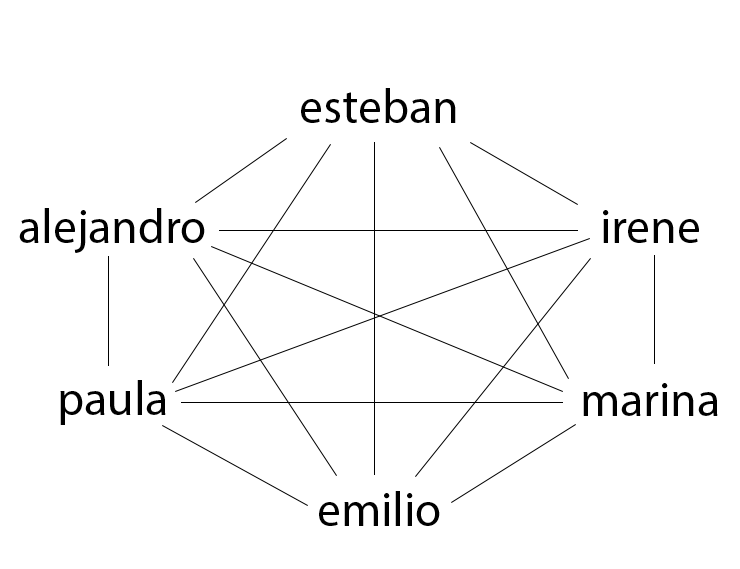
\includegraphics[width=130pt]{./figs/todosVStodos.png}
	\caption{Aquí se representa el grafo correspondiente al caso de test 'AllvsAll'}
	\label{fig:tvst}
\end{figure}
\indent Teniendo en cuenta este caso y los proporcionados por la cátedra, realizamos las corridas para evaluar su tiempo de ejecución.
\begin{center}
\begin{tabular}{|c|c|}
  \hline
  Caso de test & Tiempo de ejecución de 1000 corridas $(ms)$   \\
  \hline
  1        &  11   \\
  \hline
  2        & 213\\
  \hline
  3        & 370      \\
  \hline
  4        & 350        \\
  \hline
  5  	   & 384    \\
  \hline
  6        & 665\\
  \hline
   7 	& 628        \\
  \hline  
  all vs all 	& 152        \\
  \hline
\end{tabular}
\end{center}

\indent En la tabla los casos 1-7 representan los casos del archivo $tp1ej2.in$.\\
\indent Podemos observar claramente como influye que la complejidad es \Gather{O(k)*O(a) = O(cantidad\ de\ investigadores)*O(cantidad\ de\ amistades)} en el tiempo de ejecución. \\
\indent Esto lo podemos ver como un claro ejemplo en el caso 1 adonde al no tener amistades tenemos un tiempo de muy bajo de solo $11ms$.
En cambio en los casos que mas investigadores y amistades tienen (casos 6 y 7) son los que mas tardan si los comparamos con los casos 1-5 que no tienen tantos investigadores/relaciones.
